\documentclass[aspectratio=169,t]{beamer}
%\documentclass[aspectratio=43,t,handout]{beamer}

\usepackage[ansinew]{inputenc}
\usepackage[T1]{fontenc}
%English version FAU Logo
\usepackage[english]{babel}
%German version FAU Logo
%\usepackage[ngerman]{babel}
\usepackage{amsmath,amssymb}
\usepackage{graphicx}
\usepackage{listings}
\usepackage[backend=biber,sorting=none,doi=true,style=ieee]{biblatex}

% Themes:
%  - fau:          FAU theme
%  - fau-med:      MedFak FAU theme
%  - fau-nat:      NatFak FAU theme
%  - fau-phil:     PhilFak FAU theme
%  - fau-rw:       RWFak FAU theme
%  - fau-rw-jura:  RWFak FB Jura FAU theme
%  - fau-rw-wiso:  RWFak FB WISO FAU theme
%  - fau-tf:       TechFak FAU theme
%
% Options:
%  - image:        Cover image on title page
%  - plain:        Plain title page
%  - longtitle:    Title page layout for long title
\usetheme[longtitle]{fau-tf}

% Enable semi-transparent animation preview
\setbeamercovered{transparent}


\lstset{%
  language=C++,
  tabsize=2,
  basicstyle=\tt\scriptsize,
  keywordstyle=\color{blue},
  commentstyle=\color{green!50!black},
  stringstyle=\color{red},
  numbers=left,
  numbersep=0.5em,
  numberstyle=\tt\tiny
}


\defbibheading{bibliography}{}
\addbibresource[label=primary]{references.bib}
\nocite{*}


% Title, authors, and date
\title[Value/Proposition Canvas]{Value/Proposition Canvas for blindAR}
\subtitle{Sub Title}
\author[blindAR]{blindAR}
% English version
\institute[Innovation Lab]{Innovation Lab, Friedrich-Alexander University of Erlangen-Nuremberg}
% German version
%\institute[Lehrstuhl f\"ur XYZ]{Lehrstuhl f\"ur XYZ, Friedrich-Alexander-Universit\"at Erlangen-N\"urnberg}
\date{\today}
% Set additional logo (overwrites FAU seal)
\logo{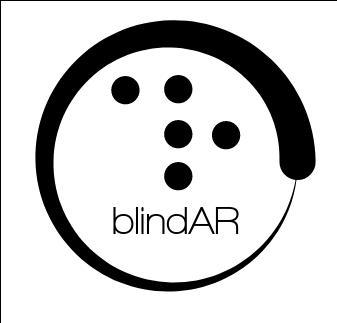
\includegraphics[width=.15\textwidth]{themefau/art/logo.png}}


\begin{document}
  % Title
  \maketitle

  %{ % Motivation
    %\setbeamertemplate{footline}{}
    %\begin{frame}[noframenumbering]{Motivation}
      %Some motivational example\dots
    %\end{frame}
  %}

  %{ % Outline
    %\setbeamertemplate{footline}{}
    %\begin{frame}[noframenumbering]{Outline}
      %\tableofcontents
    %\end{frame}
  %}

	\begin{frame}
	\frametitle{Customer Jobs}
	\begin{itemize}
		\item
			Use embedded devices with touch screens
	\end{itemize}
\end{frame}


\begin{frame}
	\frametitle{Pains}
	\begin{itemize}
		\item
			Using touch screens as a blind person is error prone
		\item
			Thus being dependent on other persons
		\item
			Exclusion
	\end{itemize}
	\vfill
	\begin{itemize}
		\item[$\Rightarrow$]
			Everyday problem!
	\end{itemize}
\end{frame}

\begin{frame}
	\frametitle{Gains}
	\begin{itemize}
		\item
			Ability to use touch screens and get coffee, train tickets, \dots
		\item
			Inclusion
		\item
			Independency
	\end{itemize}
\end{frame}

\begin{frame}
	\frametitle{Products \& Services}
	\begin{itemize}
		\item
			Software for HoloLens
		\item
			Allowing use of touch screens
			\begin{itemize}
				\item
					Vision independent
				\item
					Guided
				\item
					Interactive
			\end{itemize}
		\item
			Device independent
		\item
			Easy to extend
	\end{itemize}
\end{frame}


\begin{frame}
	\frametitle{Pain Relievers}
	\begin{itemize}
		\item
			Error free usage of touch screens
		\item
			Gain Flexibility and Independence
		\item
			Inclusion
	\end{itemize}
\end{frame}

\begin{frame}
	\frametitle{Gain Creators}
	\begin{itemize}
		\item
			Makes life easier
		\item
			Improved life quality
	\end{itemize}
\end{frame}

\logo{}
  { % Motivation
    \setbeamertemplate{footline}{}
		\begin{frame}[noframenumbering]{}

			\vspace{1.5cm}
			\centering
	\vspace{1cm}

	
\includegraphics[height=0.3\textheight]{innolab2.png}
	\hspace{1cm}
	
\includegraphics[height=0.3\textheight]{themefau/art/logo_bold.pdf}

    \end{frame}
  }
%\begin{frame}
	%\vspace{2.3cm}
	%%\vspace{1.5cm}
	%%\hspace{3cm}
	%\hspace{0.5cm}
	%
\includegraphics[height=0.3\textheight]{themefau/art/tf/fau-logo-english.pdf}
	%\hspace{0.5cm}
	%
\includegraphics[height=0.3\textheight]{innolab2.png}
	%\hspace{0.5cm}
	%%\hfill
	%
\includegraphics[height=0.3\textheight]{themefau/art/logo_bold.pdf}
%\end{frame}


\end{document}

